\section{Evaluation}
\label{sec:evaluation}
\subsection{Settings}
In order to evaluate the performance of our algorithms, we implemented them and a version of the IM-SUM algorithm from~\cite{basat2017optimal}. We evaluated the algorithms on the newest CAIDA Anonymized Internet Traces Dataset, the CAIDA`19 New-York dataset~\cite{CAIDA2019}.

For all of the evaluation, unless stated otherwise, we used the following: (1) IPv4 5-tuple flows with $|flow\_id|=104$, (2) HH threshold, $\phi=0.001$, (3) $\delta=0.05$, (4) each datapoint is the average of 10 runs, each starting in a random packet in the trace, (5) the \sea\ memory is 1\% of the available memory ($m_{SEA}=0.01)$ and (6) a propagation parameter, $v=0.35$.

To measure the performance of algorithms we used the following metrics:
\begin{itemize}
    \item Detection Rate (DR), the same as the previously mentioned Recall - which is the ratio of HH flows that the algorithm detected.
    \item False Positive Ratio (FPR) - which is the ratio of non HH flows reported by the algorithm as HH from the total number of reported flows.
    \item Throughput - the number of insertions the algorithm can perform per a single millisecond.
\end{itemize}

To be able to compare the algorithms we set the total memory available to use and the accuracy parameter. The memory usage of the IM-SUM algorithm is determined by the accuracy parameter, $\epsilon$, and its performance parameter, $\gamma$, which tunes the algorithm's memory-speed trade off.
In each run of IM-SUM, the amount of memory and the accuracy parameter was set, and we calculated the appropriate $\gamma$ for this run. For the \cs\ algorithm, the only tuning parameter is the partition of the left 99\% of the memory between the \cs\ and the \sfa\ ,i.e., setting $m_{CS}$ and $m_{SFA}=0.99-m_{CS}$.

The \cs\ algorithm and the IM-SUM algorithm provide different accuracy guarantees on the reported set of flows. The IM-SUM algorithm ensures accuracy in the range $[N(\phi-\epsilon),N \phi]$ while the \cs\ algorithm ensures accuracy in the range $[(1-\delta)\phi N, \phi N]$. The effective accuracy slack of the IM-SUM algorithm is $N\epsilon$, which is much larger than \cs's slack of $N\delta\phi$. Thus when comparing the algorithms with the same accuracy parameter, $\epsilon=\delta$, we give an edge to the IM-SUM algorithm, allowing it to possibly report more flows as HH than the \cs\ algorithm.

\subsection{Results}

\begin{figure*}
\begin{subfigure}[t]{0.32\textwidth}
    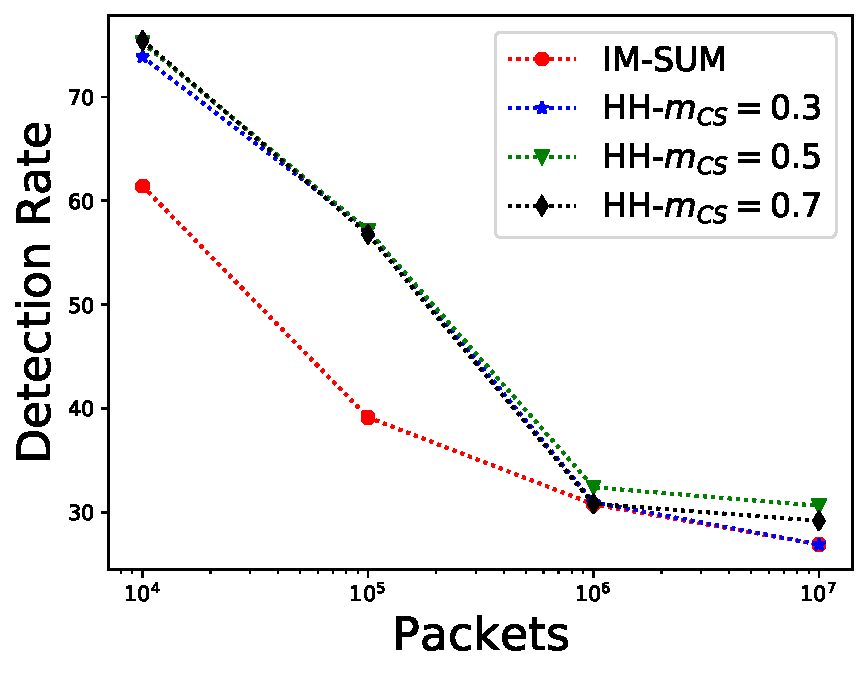
\includegraphics[width=\linewidth]{HH/figures/DR_per_pkts_m=0.03125.pdf}
    \caption{32KB}
    \label{fig:fig2_a}    
\end{subfigure}\hfill
\begin{subfigure}[t]{0.32\textwidth}
    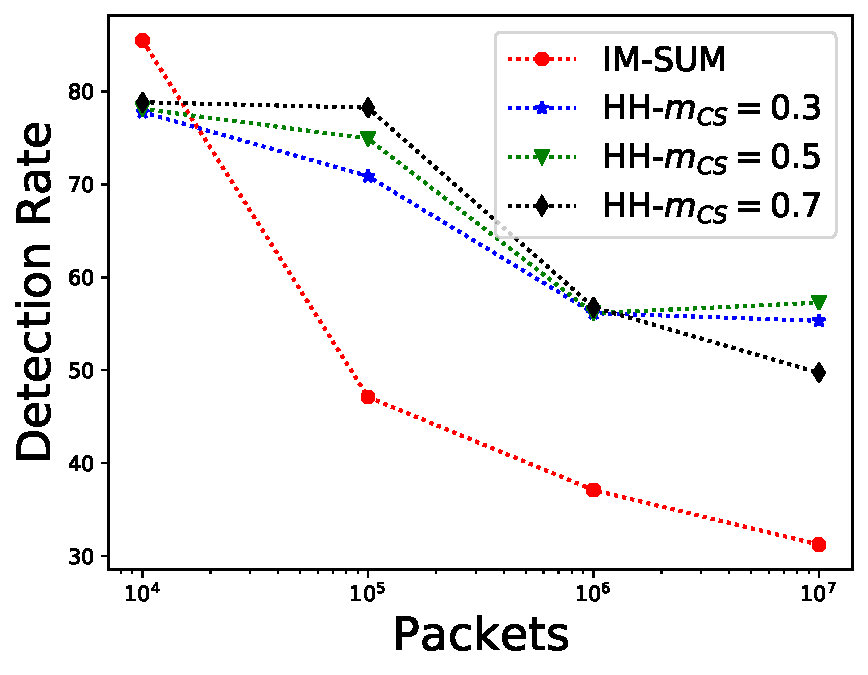
\includegraphics[width=\linewidth]{HH/figures/DR_per_pkts_m=0.0625.pdf}
    \caption{64KB}
    \label{fig:fig2_b}
\end{subfigure}\hfill
\begin{subfigure}[t]{0.32\textwidth}
    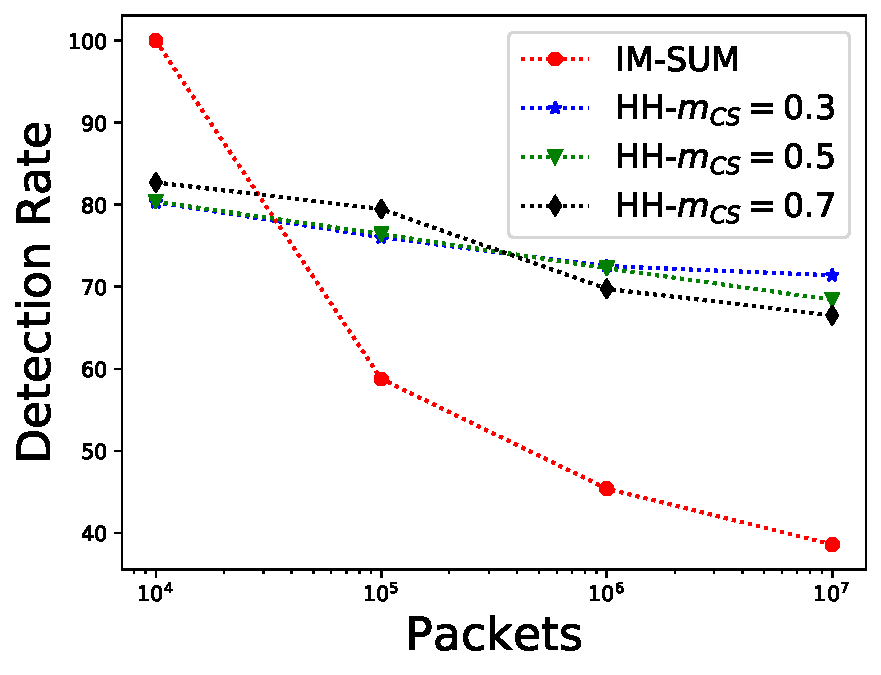
\includegraphics[width=\linewidth]{HH/figures/DR_per_pkts_m=0.125.pdf}
    \caption{128KB}
    \label{fig:fig2_c}
\end{subfigure}

\begin{subfigure}[t]{0.32\textwidth}
    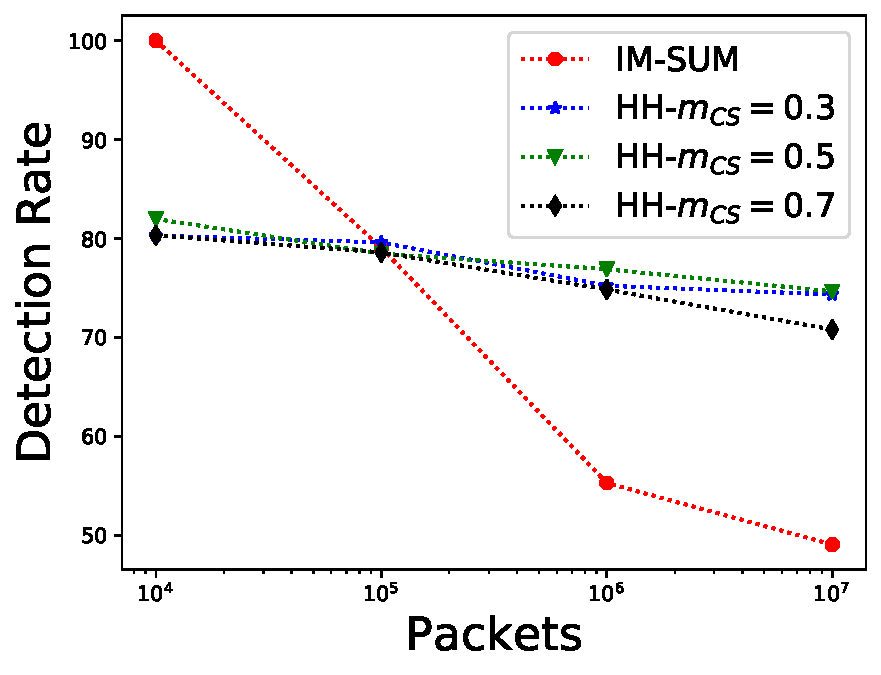
\includegraphics[width=\linewidth]{HH/figures/DR_per_pkts_m=0.25.pdf}
    \caption{0.25MB}
    \label{fig:fig2_d}
\end{subfigure}\hfill
\begin{subfigure}[t]{0.32\textwidth}
    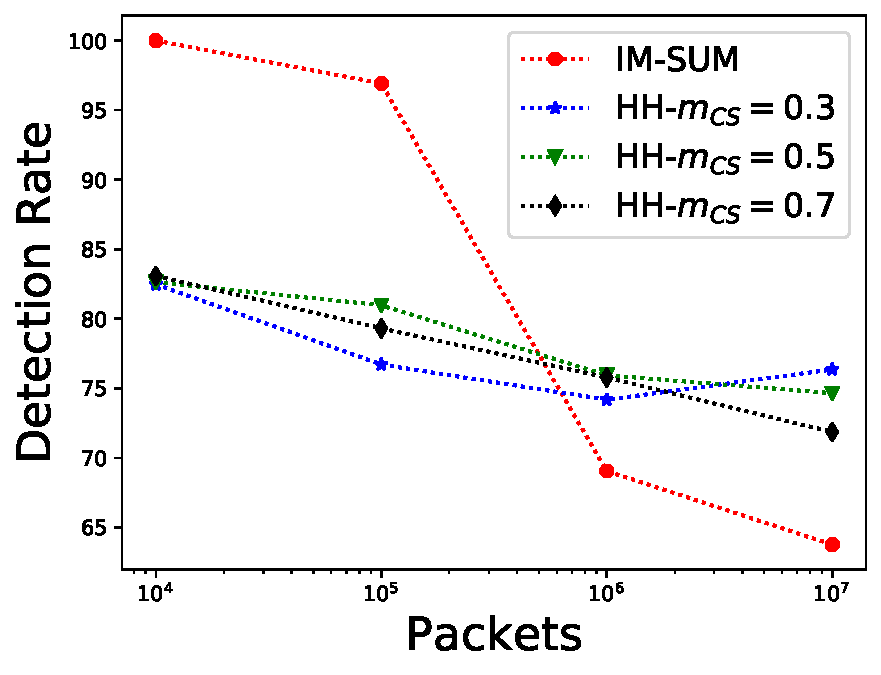
\includegraphics[width=\linewidth]{HH/figures/DR_per_pkts_m=0.5.pdf}
    \caption{0.5MB}
    \label{fig:fig2_e}
\end{subfigure}\hfill
\begin{subfigure}[t]{0.32\textwidth}
    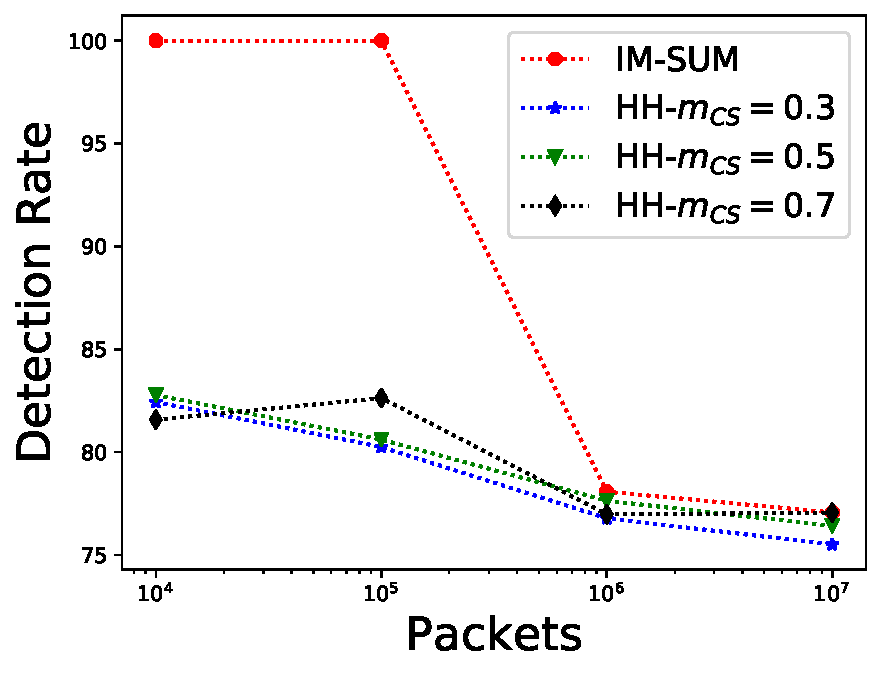
\includegraphics[width=\linewidth]{HH/figures/DR_per_pkts_m=1.0.pdf}
    \caption{1MB}
    \label{fig:fig2_f}
\end{subfigure}

\caption{The Average Detection Rate as function of number of packets, comparing our algorithm in three different settings vs. the Elephants algorithm for $\phi=0.001,\delta=0.05$}
\label{figure2}
\end{figure*}


Figures~\ref{fig:fig2_a}-~\ref{fig:fig2_f} show the average DR of the algorithms as a function of the number of packets processed. Intuitively, the DR relies heavily on the amount of available memory and one can see that the more memory allocated to the algorithms, the higher the DR rate is. When evaluating the \cs\ algorithm, we tested several variants with the different partition of the memory between the \cs\ and the \sfa. These variants allocates 30\%,50\%,70\% of the memory to the \cs\ and 69\%,49\%,29\% to the \sfa\ accordingly.

It is not clear how this trade off between the size of the \cs\ and the size of the \sfa\ affects the performance of the algorithm. When \cs\ is large the algorithm can hold on to ``big" flows while when  \sfa\ is large the algorithm can hold on to the more ``recent" flows. One can see that while the partition is balanced enough, that means there are no too few entries in the \sfa\ nor in the \cs\ and the effect on DR is small.

Figures~\ref{fig:fig2_a} and~\ref{fig:fig2_b} show that the \cs\ performs better than IM-SUM algorithm for amounts of memory smaller than 64KB and in some settings even finds 50\% more HH flows. However, it is worthy to note that, that both algorithm's DR degrades when processing more packets in this range of memories, which is unexpected since none of the algorithms guarantees relies on $N$.
Figures~\ref{fig:fig2_c} to~\ref{fig:fig2_f} show that this phenomenon of DR degradation when the number of packets increase is not present in the \cs\ algorithm compared to the IM-SUM algorithm.

However, this is not the case for the IM-SUM algorithm. The more memory the algorithm has the higher the DR, while the more packets processed the lower the DR. That is, for a given amount of memory our algorithm can process more packets without compromising its DR.

\begin{figure*}
\begin{subfigure}[t]{0.32\textwidth}
    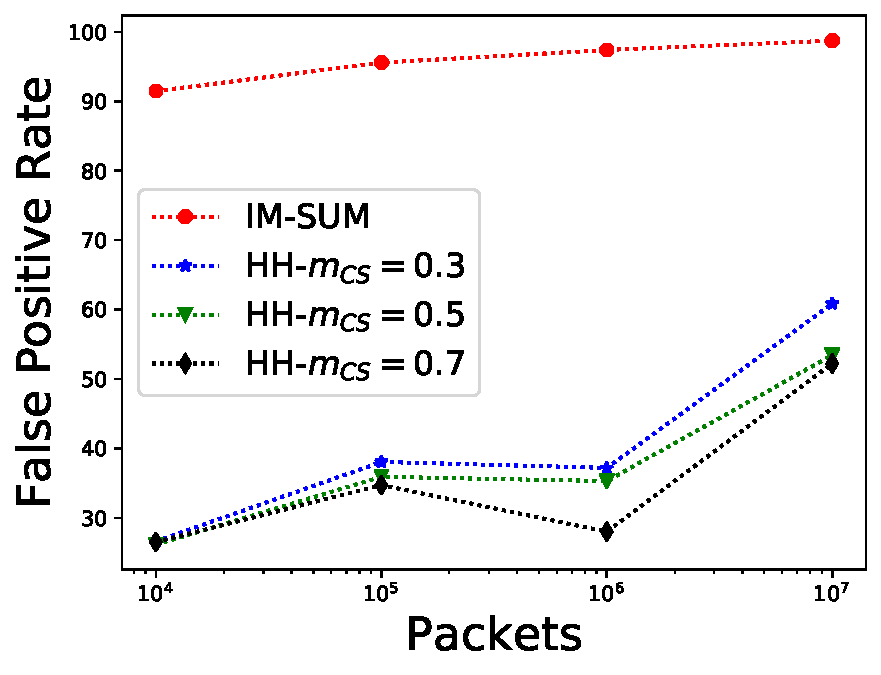
\includegraphics[width=\linewidth]{HH/figures/FPR_per_pkts_m=0.03125.pdf}
    \caption{32KB}
    \label{fig:fig3_a}    
\end{subfigure}\hfill
\begin{subfigure}[t]{0.32\textwidth}
    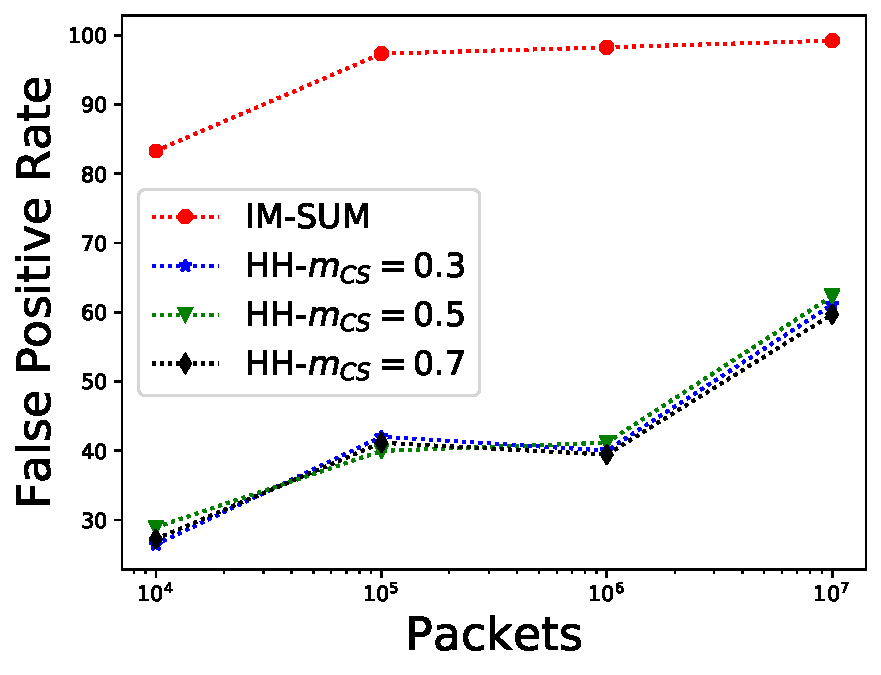
\includegraphics[width=\linewidth]{HH/figures/FPR_per_pkts_m=0.0625.pdf}
    \caption{64KB}
    \label{fig:fig3_b}
\end{subfigure}\hfill
\begin{subfigure}[t]{0.32\textwidth}
    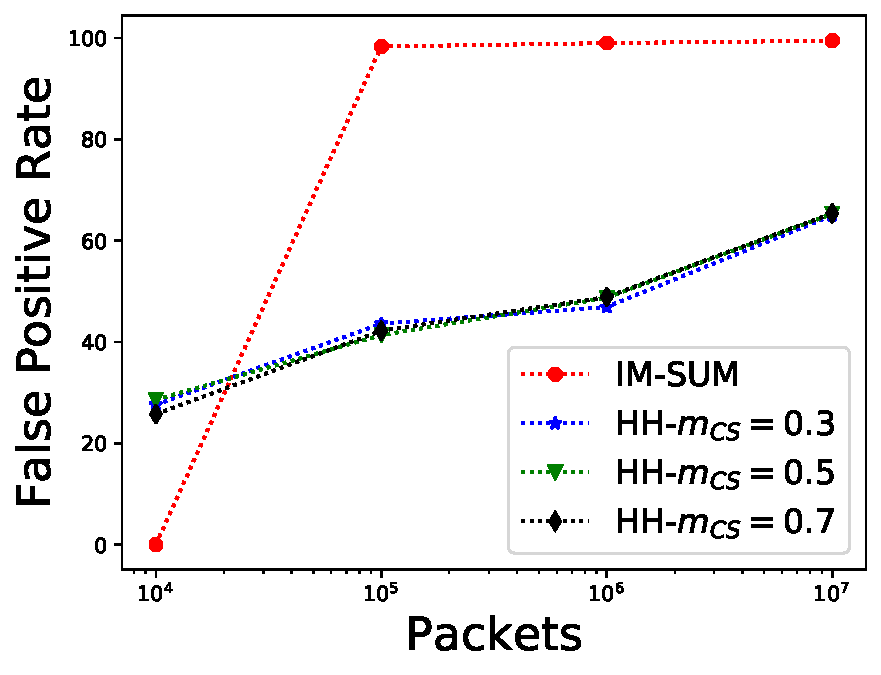
\includegraphics[width=\linewidth]{HH/figures/FPR_per_pkts_m=0.125.pdf}
    \caption{128KB}
    \label{fig:fig3_c}
\end{subfigure}

\begin{subfigure}[t]{0.32\textwidth}
    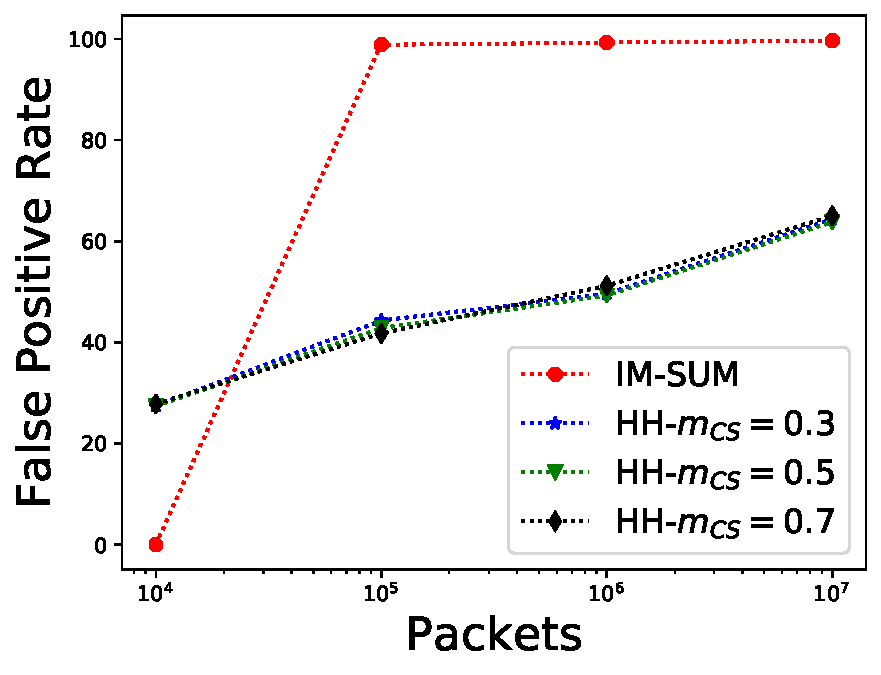
\includegraphics[width=\linewidth]{HH/figures/FPR_per_pkts_m=0.25.pdf}
    \caption{0.25MB}
    \label{fig:fig3_d}
\end{subfigure}\hfill
\begin{subfigure}[t]{0.32\textwidth}
    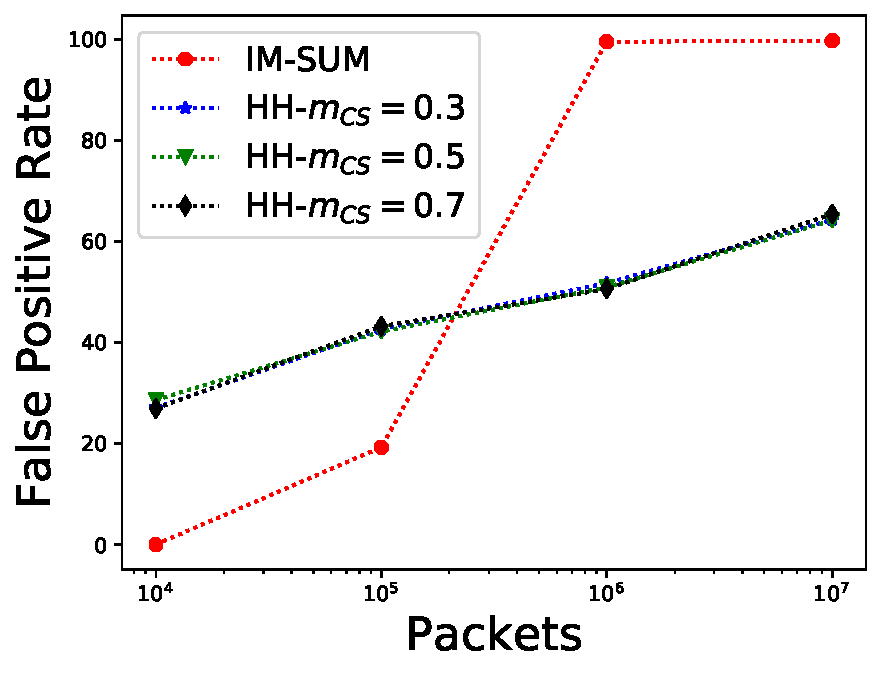
\includegraphics[width=\linewidth]{HH/figures/FPR_per_pkts_m=0.5.pdf}
    \caption{0.5MB}
    \label{fig:fig3_e}
\end{subfigure}\hfill
\begin{subfigure}[t]{0.32\textwidth}
    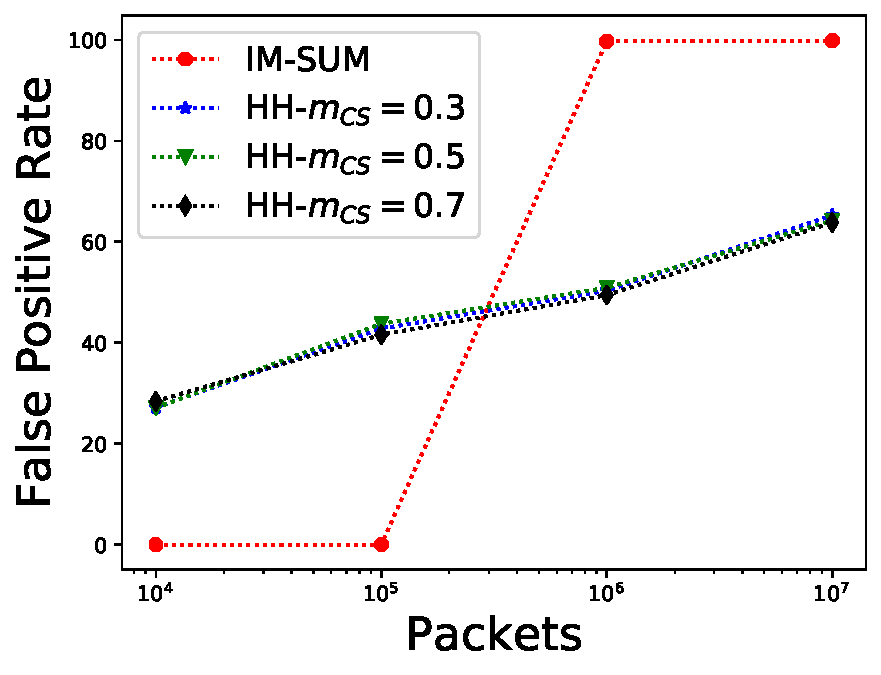
\includegraphics[width=\linewidth]{HH/figures/FPR_per_pkts_m=1.0.pdf}
    \caption{1MB}
    \label{fig:fig3_f}
\end{subfigure}

\caption{The Average False Positive Rate as function of number of packets, comparing our algorithm in three different settings vs. the Elephants algorithm for $\phi=0.001,\delta=0.05$}
\label{figure3}
\end{figure*}

Figures~\ref{fig:fig3_a}-~\ref{fig:fig3_f} show the average FPR of the algorithms as a function of the number of packets processed. It is worthy to note that the FPR of the \cs\ algorithm does not depend on the amount of memory, that is, using more memory does not affect the FPR. This is true since the algorithm's FPR depends directly on the estimation given by the \sea, and this estimation is always accurate up to $1\pm \delta$, regardless of the amount of memory. This also explains the lack of effect of the value of $m_{CS}$ on the FPR.

Interestingly, when the IM-SUM algorithm is given enough memory and not many packets, it will not report false positive flows. However, for each memory settings there is a number of packets where the algorithm starts reporting almost 100\% false positive flows, this means that the vast majority of the reported set of flows is non HH flows.

When considering the comparison of the algorithms in terms of FPR, it is evident that the \cs\ algorithm performs better. For less than $64KB$ it is always less than IM-SUM's FPR, while for larger amounts of memory it stays pretty constant in the range 40\%-60\% while IM-SUM's FPR soars quickly to around 100\%.

\begin{figure*}

\begin{subfigure}[t]{0.32\textwidth}
    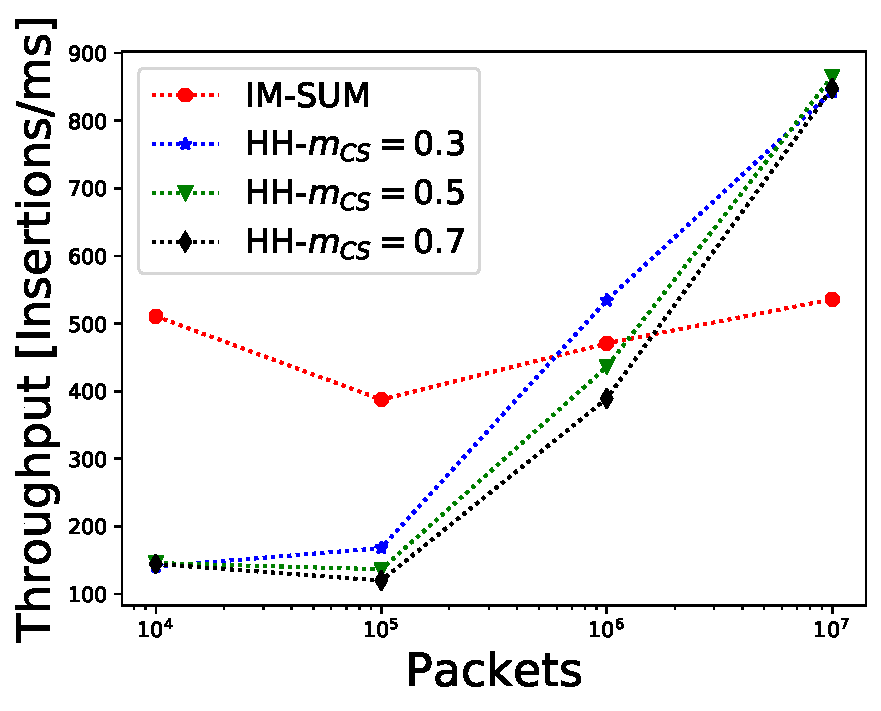
\includegraphics[width=\linewidth]{HH/figures/throughput_per_pkts_m=0.03125.pdf}
    \caption{32KB}
    \label{fig:fig4_a}    
\end{subfigure}\hfill
\begin{subfigure}[t]{0.32\textwidth}
    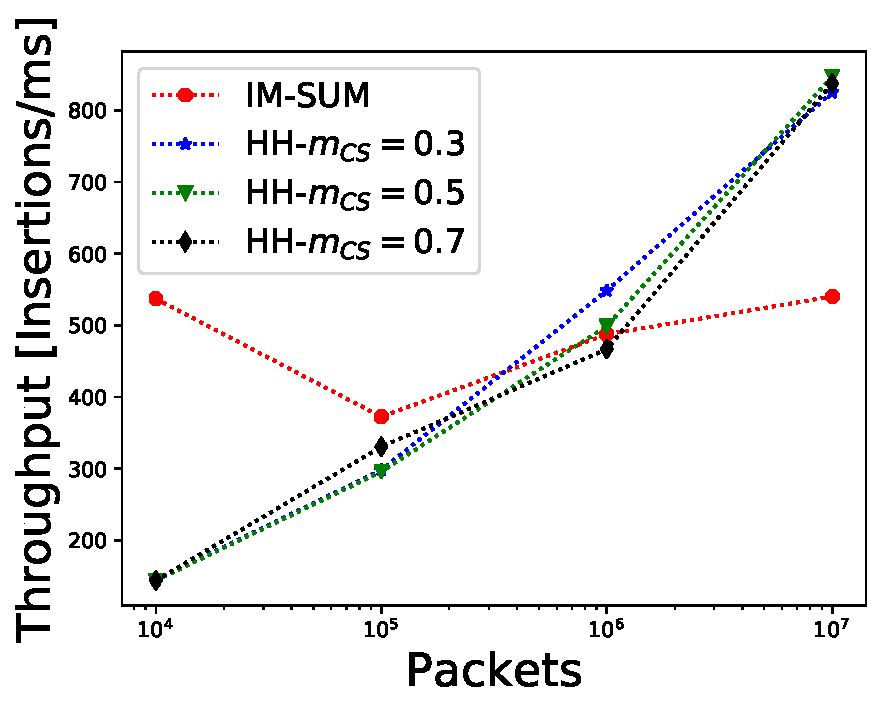
\includegraphics[width=\linewidth]{HH/figures/throughput_per_pkts_m=0.0625.pdf}
    \caption{64KB}
    \label{fig:fig4_b}
\end{subfigure}\hfill
\begin{subfigure}[t]{0.32\textwidth}
    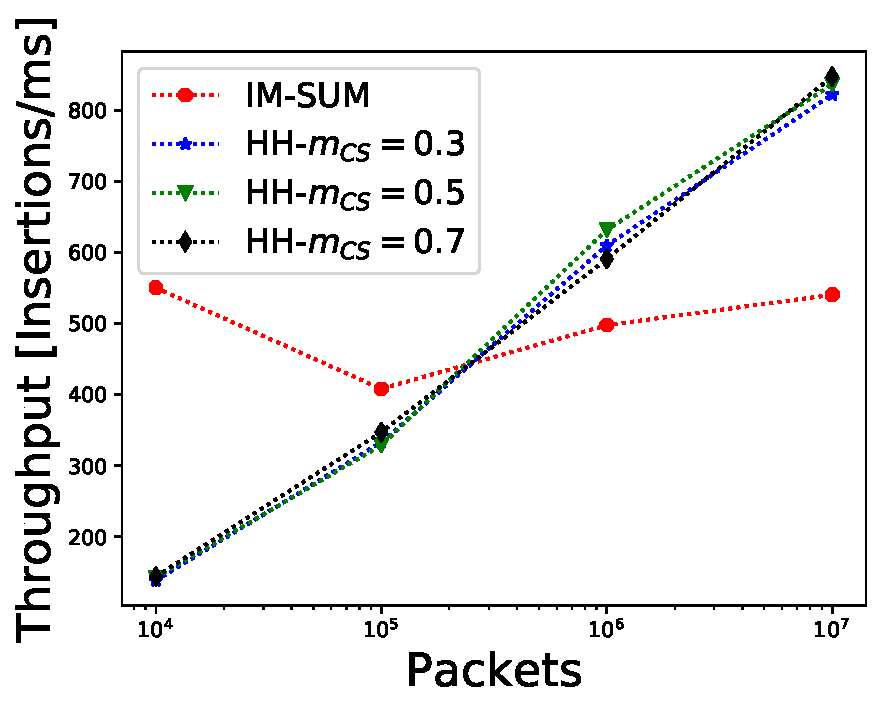
\includegraphics[width=\linewidth]{HH/figures/throughput_per_pkts_m=0.125.pdf}
    \caption{128KB}
    \label{fig:fig4_c}
\end{subfigure}

\begin{subfigure}[t]{0.32\textwidth}
    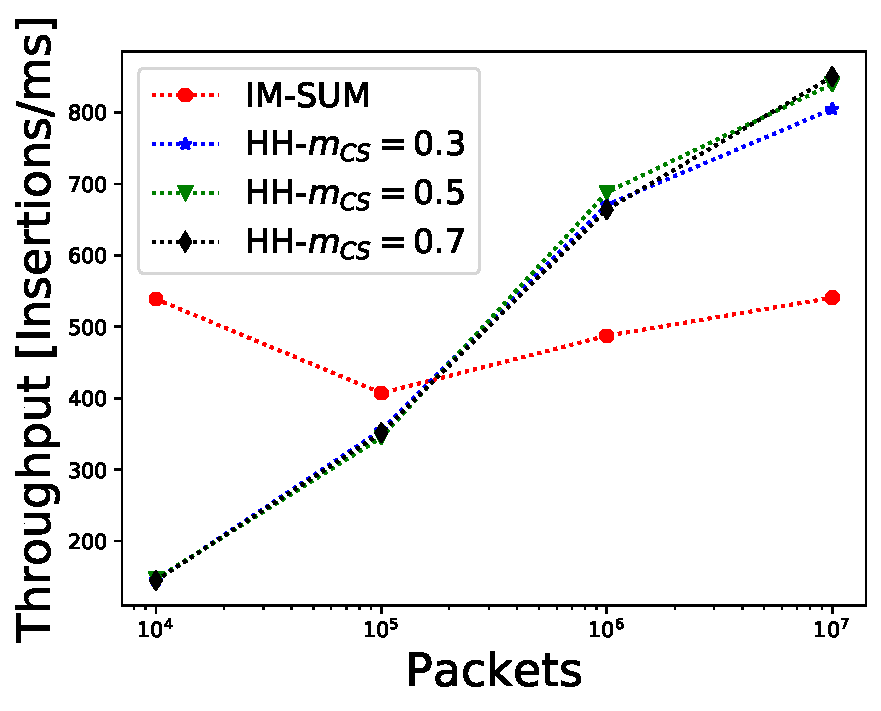
\includegraphics[width=\linewidth]{HH/figures/throughput_per_pkts_m=0.25.pdf}
    \caption{0.25MB}
    \label{fig:fig4_d}
\end{subfigure}\hfill
\begin{subfigure}[t]{0.32\textwidth}
    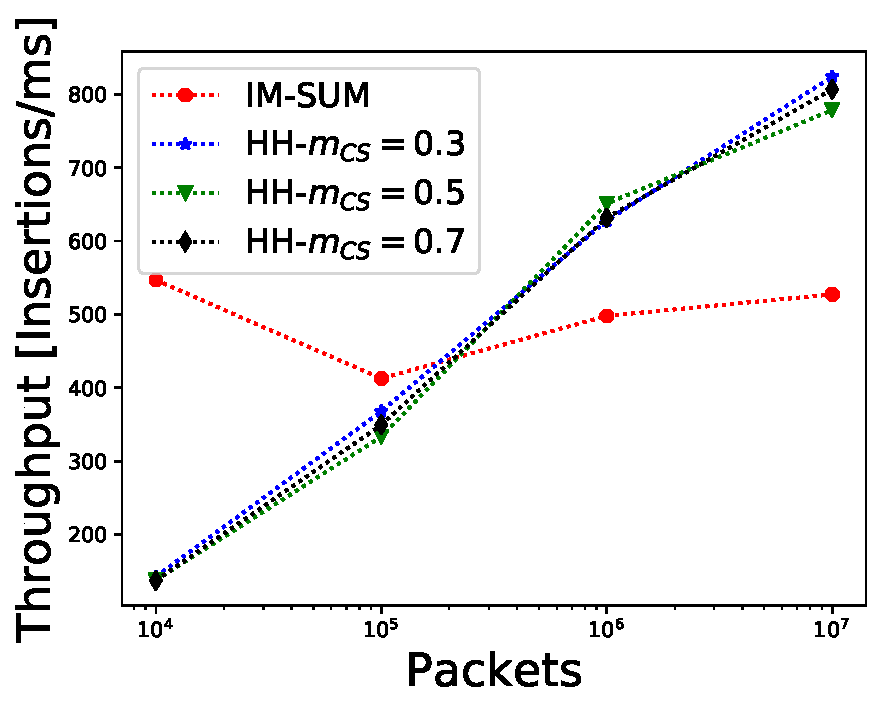
\includegraphics[width=\linewidth]{HH/figures/throughput_per_pkts_m=0.5.pdf}
    \caption{0.5MB}
    \label{fig:fig4_e}
\end{subfigure}\hfill
\begin{subfigure}[t]{0.32\textwidth}
    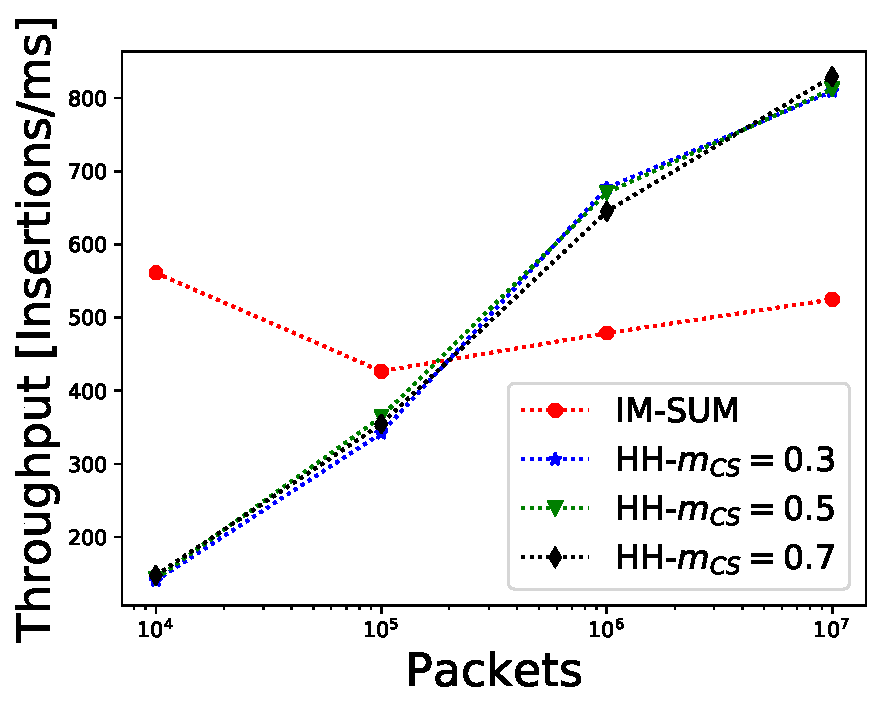
\includegraphics[width=\linewidth]{HH/figures/throughput_per_pkts_m=1.0.pdf}
    \caption{1MB}
    \label{fig:fig4_f}
\end{subfigure}

\caption{The Average Throughput as function of number of packets, comparing our algorithm in three different settings vs. the Elephants algorithm for $\phi=0.001,\delta=0.05$}
\label{figure4}
\end{figure*}

Figures~\ref{fig:fig4_a}-~\ref{fig:fig4_f} show the throughput in terms of insertions per millisecond of the algorithms as a function of the number of packets processed. For both algorithms, the more packets processed for a given amount of memory, the higher the throughput. In the case of IM-SUM, it seems that for $N=10^4$ we get the highest throughput. However, this datapoint is an anomaly since, with that few packets, the algorithm does not perform the heavy maintenance operation.

In the case of the \cs\ algorithm, the more packets we process the higher the throughput due to the fact that more packets yields higher $v_0$ and higher values in the \sea. This is translated to fewer operations per packet since its insertion is probabilistic with an inverse relation to the values in the \sea. This is also supported by the fact that the \cs\ algorithm performs $O(1)$ ``maintenance" operations compared to IM-SUM amortized maintenance operation.

It is worth to note that the throughput of our algorithm is not affected by the amount of memory, that is true since all of the accesses to the data structures are $O(1)$ and does not rely on the sizes of these data structures.

\begin{figure}
    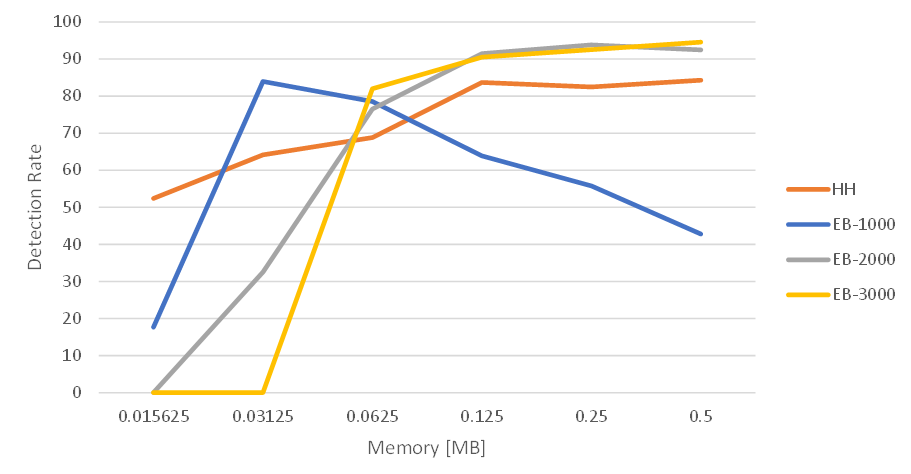
\includegraphics[width=\linewidth]{HH/figures/EB.png}
    \caption[Average Detection Rate of \cs\ and the \eb\ algorithms]{The Average Detection Rate as function of memory, comparing our the \cs\ algorithm and the \eb\ algorithm with different sizes of banks ($\phi=0.001,\delta=0.05m N=10^7, m_{CS}=0.5, m_{SEA}=0.01$)}
    \label{figure5}
\end{figure}

Figure~\ref{figure5} compares the DR of the \cs\ algorithm with the \eb\ algorithm with three sizes of banks 1000, 2000, and 3000. Since every 1000 entries in the \eb\ algorithm require around $16KB$, the algorithm suffers from poor DR in the smaller ranges of the memory. However, once the memory allows a decent size of the \sfa, the \eb\ algorithm starts to perform better since many more HH flows are propagating to the bank and have now an exact estimation up to the \pe\ introduced by the \sfa. One should note, that for \eb\ with size 1000 the DR becomes poor once again the larger the \sfa, that is since larger \sfa\ is propagating too many flows to the \eb\ and without an eviction. It is important to note, this higher DR comes with a cost of lower throughput and higher FPR since it performs a linear search in the size of the bank (which is constant) and it returns all flows in the \eb\ as potential HH.